
\documentclass[10pt]{article}
\usepackage[utf8]{inputenc}
\usepackage{kotex}
\usepackage{graphicx}
\usepackage{subfigure}
\usepackage{titling}
\setlength{\droptitle}{-2cm}
\usepackage{array}
\usepackage{amssymb}
\usepackage{amsmath}
\usepackage{siunitx} 
\usepackage{enumerate} 
\usepackage{pgfplots}
\usepackage{pgfplotstable}
\usepackage{tikz,pgfplots}
\usepackage{wasysym}
\usepackage{geometry}
\usepackage{authblk}
\usepackage{kotex}
\usepackage{bibunits}
\usepackage{tabularx}
\usepackage{hyperref}
\usepackage{pythonhighlight}

\geometry{
    a4paper,
    total={170mm,257mm},
    left=20mm,
    top=20mm,
}

\title{\textbf{Mathematical Foundation of DNN : HW 2}}
\author{Jeong Min Lee}

\begin{document}
\maketitle
In this assigment, I implemented every algorith both with torch package and without it(except problem 7). 
I'll focus on the result of optimization and the comparison both implmentations. Also, I attached the code what I used in this assignment in appendix of this document. Please refer to it.
\section{}

I refer the code given by lecture to implement the SGD with logistic regression. The result of this code is 
described in figure \ref{fig1}. As figure \ref{fig1} depicted, both implementation succeeded convergence, since their losses were decreasing and saturated.
Since the algorithm without torch and optimizer is too naive, the performace of SGD without SGD is worse than that with torch. To be specific, 
the result drawn by SGD without torch has larger loss and sizeable variance. I guess the optimizer torch using is more sophisticated and effective. 

\begin{figure}[!h]
    \begin{center}
        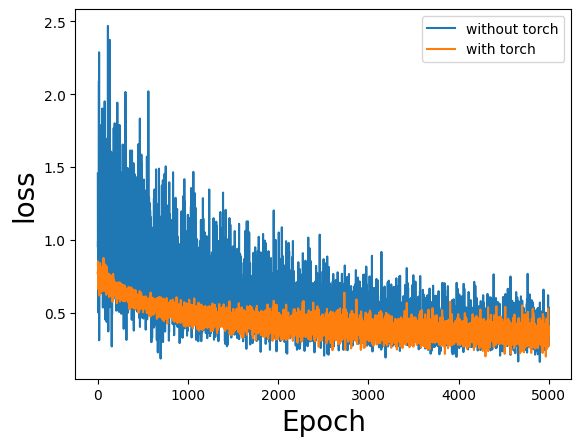
\includegraphics[scale = 0.5]{../hw2/fig/prob1.png}
        \label{fig1}
    \end{center}
    \caption{The comparison of the algorithm of SGD both with torch and without it.}
\end{figure}

\section{}
Simiar to problem 1, both algorithm were successful to converge. Surprisingly, in this problem, my own SGD algorithm outperform the implementation with torch.
I conjecture that this outperformace is intrinsic algorithmic issues in torch or the hyperparameter tuning. At the first, I suspect that the SGD in torch hit the non-differentiable point of ReLU function.
However, when I counted the number of hit that SGD meet the non-differential point within its training, it result in zero, that is, SGD never meet non-differentiable point in its training process. 
Even if the implementation with torch cannot show good performance, 
it still better than logistic regression.

\begin{figure}[!h]
    \begin{center}
        \subfigure[]{
            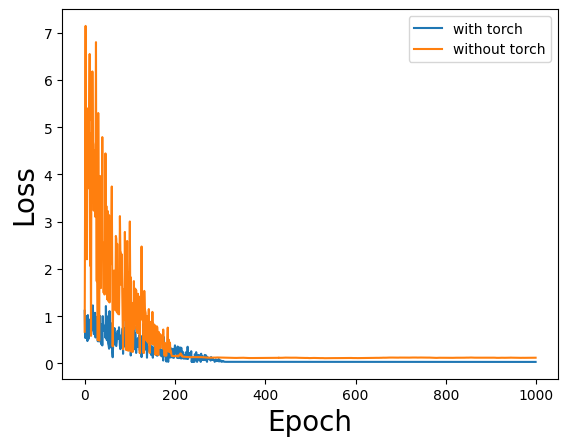
\includegraphics[scale = 0.5]{../hw2/fig/prob2.png}
        }
        \subfigure[]{
            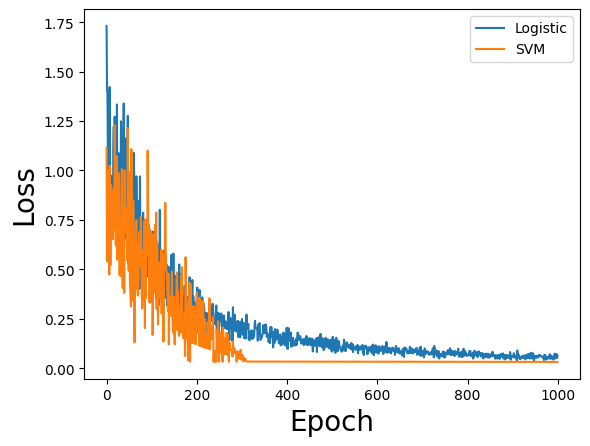
\includegraphics[scale = 0.5]{../hw2/fig/prob2_2.png}
        }
        \label{fig2}
    \end{center}
    \caption{(a) The comparison of the algorithm of SGD both with torch and without it. (b) The comparision between logistic regression and SVM.}
\end{figure}


\section{}

As one can check from figure \ref{fig3}, the given data is not linearly separable, that is, there is no line that separate both red and blue dot into two sectors.
However, after transform the $X$ using $\varphi$, this data can be linearly separable. To calculate the decision boundary, I used SVM which is more superior than logistic regression.

\begin{figure}[!h]
    \begin{center}
        \subfigure[]{
            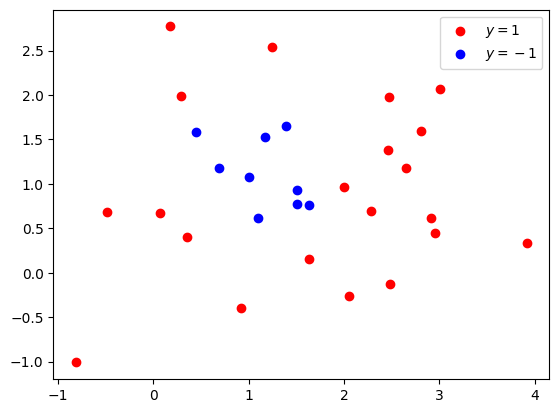
\includegraphics[scale = 0.5]{../hw2/fig/prob3.png}
        }
        \subfigure[]{
            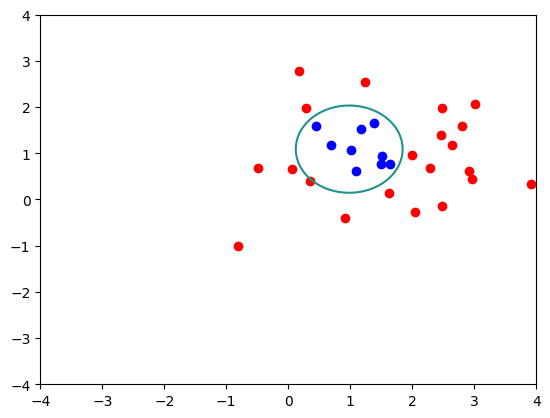
\includegraphics[scale = 0.5]{../hw2/fig/prob3_2.png}
        }
    \end{center}
    \caption{(a) The scatter plot of given data with its label. (b) The scatter plot with decision boundary(green) obtained by SVM.}
    \label{fig3}
\end{figure}


\section{}
\textbf{CLAIM} : $y = -\log(x)$ function is strict convex function. 
To prove the \textbf{CLAIM} above, I proved the following \textbf{LEMMA}.


\textbf{LEMMA} : The differentiable function $f$ is strictly convex \textit{if and only if} its derivate $f^\prime$ is strictly increasing.
\textbf{proof}\\
$\implies :     a,b \in \mathbb{R} (a<b). \text{Let} x_1, x_2, x_3 \in \mathbb{R} \text{ be chosen s.t. } a<x_1<x_2<x_3<b.$

From Chordal Slope Lemma, which is famous lemma applicable to convex function,

\begin{equation}
    \frac{f(x_1) - f(a)}{x_1 - a} < \frac{f(x_2) - f(x_1)}{x_2 - x_1}<\frac{f(x_3) - f(x_2)}{x_3 - x_2} < \frac{f(b) - f(x_3)}{b - x_3}
    \label{eqn1}
\end{equation} 
\begin{equation}
    \frac{f(x_2) - f(a)}{x_2 - a} < \frac{f(b) - f(x_2)}{b - x_2}
\end{equation} 

Taking limit $x_1 \rightarrow a, x_3 \rightarrow b$ on equation \ref{eqn1}, 

\begin{equation}
    f^\prime(a) \le \frac{f(x_2) - f(a)}{x_2 - a} < \frac{f(b) - f(x_2)}{b - x_2} \le f^\prime(b)
\end{equation}\\
$\Longleftarrow$ : Let $x_1, x_2, x_3 \in \mathbb{R}$ s.t. $x_1<x_2<x_3$. From Mean Value Theorem,
\begin{equation}
    \exists a \text{ s.t } \frac{f(x_2) - f(x_1)}{x_2 - x_1} = f^\prime(a) \\
\end{equation}
\begin{equation}
    \exists b \text{ s.t } \frac{f(x_3) - f(x_2)}{x_3 - x_2} = f^\prime(b)
\end{equation}
Note that $x_1<a<x_2<b<x_3$. Since $f^\prime$ is strictly increasing, $f^\prime(a) < f^\prime(b)$, which implies 
\begin{equation}
    \frac{f(x_2) - f(x_1)}{x_2 - x_1} < \frac{f(x_3) - f(x_2)}{x_3 - x_2} 
    \label{eqn6}
\end{equation}
The result of equation \ref{eqn6} is equivalent that $f$ is strictly convex according to Chordal Slope Lemma.$\blacksquare$ 

\textbf{proof of CLAIM}
From the Lemma prove above, it is enough to show that the derivative of $y = -\log(x)$ is strictly increasing. 
\begin{equation}
    {d^2 \over dx^2} \left(-\log(x)\right) = \frac{1}{x^2} >0 \text{ for } x>0
\end{equation}
Since the second derivative of $f(x) = -\log(x)$ is positive definite within the region that logarithm is defined. 
This implies that $f^\prime$ is strictly increasing.$\blacksquare$


From the claim, one can show that $D_{KL}>0$ for different probability mass function $p, q$. Furthermore, $D_{KL}=0$ \textit{if and only if} $p = q$.  

\begin{equation}
    -D_{KL}(p||q) = -\sum_i p_i\log{\frac{p_i}{q_i}} = \mathbb{E}_{p}\left[\log{\frac{q_i}{p_i}}\right] < \log{\mathbb{E}_p\left[\frac{q_i}{p_i}\right]} = \log q_i \le \log 1 = 0 
    \label{eqn8}
\end{equation}

If $p=q$, then, 
\begin{equation}
    D_{KL}(p||q) = \sum_i p_i \log{\frac{p_i}{q_i}} = \sum_i p_i \log{1} = 0
\end{equation}
Since if $p\neq q$, we can apply the formulation made in equation \ref{eqn8}, $D_{KL}$ never be zero. 
\section{}
\section{}
\section{}
\appendix

\begin{python}
import numpy as np
import torch
import torch.nn as nn
from random import randint
import matplotlib.pyplot as plt
# Hyperparameters setup and Prepare Dataset
N,p = 30,20
np.random.seed(0)
X = np.random.randn(N,p)
Y = 2*np.random.randint(2,size = N)-1
lr = 1e-4
epoch = 5000
class LR(nn.Module):
    def __init__(self,input_dim = p):
        super().__init__()
        self.linear = nn.Linear(input_dim, 1, bias = True)
    
    def forward(self, x):
        return self.linear(x)

model = LR()

def logistic_loss(output, target):
    return -torch.nn.functional.logsigmoid(target*output)

loss_function = logistic_loss                                                   
optimizer = torch.optim.SGD(model.parameters(), lr=lr) 
losses = []
for _ in range(epoch) :
    tmp_losses = []
    for _ in range(N):
        # Sampling
        idx = randint(0, N-1)
        target, label = X[idx], Y[idx]

        optimizer.zero_grad()

        train_loss = loss_function(model(torch.FloatTensor(target)), label)
        tmp_losses.append(train_loss)
        train_loss.backward() # calculate graident via backpropagation
        optimizer.step() # update the parameteres
    losses.append(np.mean([x.detach().numpy() for x in tmp_losses]))
    
\end{python}

\begin{python}
import numpy as np
from random import randint
import matplotlib.pyplot as plt
N,p = 30,20
np.random.seed(0)
X = np.random.randn(N,p)
Y = 2*np.random.randint(2,size = N)-1
lr = 1e-4
epoch = 5000
class LR():
    def __init__(self,input_dim = p):
        self.weight = np.random.uniform(0,1,input_dim+1) # last row is bias term
    def output(self,x):
        x = np.append(x,1) # add dummy column that is one
        return x.T@self.weight
    def update_weight(self,grad,lr = 1e-4):
        self.weight = self.weight - lr * grad

model = LR()

def logistic_loss(output, target):
    return np.log(1+np.exp(-target*output))

loss_function = logistic_loss                                                   
losses = []

for _ in range(epoch) :
    tmp_losses = []
    for _ in range(p):
        # Sampling
        idx = randint(0, N-1)
        target, label = X[idx], Y[idx]
        
        train_loss = loss_function(model.output(target), label)
        tmp_losses.append(train_loss)
        grad = (1-train_loss)*label*np.append(target,label)
        model.update_weight(grad,lr = lr)
    losses.append(np.mean([x for x in tmp_losses]))
\end{python}

\begin{python}
import numpy as np
import torch
import torch.nn as nn
from random import randint
import matplotlib.pyplot as plt
# Hyperparameters setup and Prepare Dataset
N,p = 30,20
np.random.seed(0)
X = np.random.randn(N,p)
Y = 2*np.random.randint(2,size = N)-1
lr = 1e-3
epoch = 500
regularizer = 0.1 # lambda
class SVM(nn.Module):
    def __init__(self,input_dim = p):
        super().__init__()
        self.linear = nn.Linear(input_dim, 1, bias = True)
    
    def forward(self, x):
        return self.linear(x)

model = SVM()
optimizer = torch.optim.SGD(model.parameters(), lr=lr) 
svm_losses = []
cnt = 0
for _ in range(epoch) :
    tmp_losses = []
    for _ in range(p):
        # Sampling
        idx = randint(0, N-1)
        target, label = X[idx], Y[idx]

        optimizer.zero_grad()
        
        train_loss = torch.clamp(1-label*model(torch.FloatTensor(target)),min = 0) + regularizer*model.linear.weight@model.linear.weight.T
        train_loss.requires_grad_(True)
        tmp_losses.append(train_loss)
        train_loss.backward() # calculate graident via backpropagation
        optimizer.step() # update the parameteres
    svm_losses.append(np.mean([x.detach().numpy() for x in tmp_losses]))
\end{python}

\begin{python}
import numpy as np
from random import randint
import matplotlib.pyplot as plt

# Hyperparameters setup and Prepare Dataset
N,p = 30,20
np.random.seed(0)
X = np.random.randn(N,p)
Y = 2*np.random.randint(2,size = N)-1
lr = 1e-3
epoch = 5000
regularizer = 0.1 # lambda

class SVM():
    def __init__(self,input_dim = p):
        self.weight = np.random.uniform(0,1,input_dim+1) # last row is bias term
        self.regularizer =regularizer
    def output(self,x):
        return x.T@self.weight
    def update_weight(self,grad,lr = 1e-4):
        self.weight = self.weight - lr * grad

    def loss_function(self, x, y):
        x = np.append(x,y)
        return np.max([0, 1-y*self.output(x)]) + self.weight@self.weight.T *regularizer
    
    def loss_prime(self, x,y):
        x = np.append(x,y)
        if y*self.output(x) <1 : 
            return -y*x +2*self.regularizer*self.weight
        else:
            return 2*self.regularizer*self.weight

model = SVM()
svm_losses = []
cnt = 0

for _ in range(epoch):
    tmp_loss = []
    for _ in range(p):
        idx = randint(0,N-1)
        input,label = X[idx], Y[idx]
        z = model.output(np.append(input,label))
        if z==1:
            cnt+=1
        train_loss = model.loss_function(input, label)
        tmp_loss.append(train_loss)
        grad = model.loss_prime(input,label)
        
        model.update_weight(grad=grad, lr = lr)
    svm_losses.append(np.mean(tmp_loss))

plt.plot(range(epoch), np.abs(svm_losses))
plt.xlabel("Epoch",fontsize = 20)
plt.ylabel("Loss",fontsize = 20)
plt.show()
print(cnt)
\end{python}

\begin{python}
for i in range(N):
    if y[i] == 1:
        plt.scatter(X[0,i],X[1,i],color = "red")
    if y[i] == -1:
        plt.scatter(X[0,i],X[1,i],color = "blue")
plt.legend(["$y = 1$","$y = -1$"])
plt.show()

def trans(x):
    return [1,x[0],x[0]**2, x[1],x[1]**2]
X_trans = np.asarray([trans(x) for x in X.T]).T # (5,N)

import numpy as np
from random import randint
import matplotlib.pyplot as plt

N,p = 30,5
lr = 1e-3
epoch = 500
regularizer = 0.1 # lambda

class SVM():
    def __init__(self,input_dim = p):
        self.weight = np.random.uniform(0,1,input_dim+1) # last row is bias term
        self.regularizer =regularizer
    def output(self,x):
        return x.T@self.weight
    def update_weight(self,grad,lr = 1e-4):
        self.weight = self.weight - lr * grad

    def loss_function(self, x, y):
        x = np.append(x,y)
        return np.max([0, 1-y*self.output(x)]) + self.weight@self.weight.T *regularizer
    
    def loss_prime(self, x,y):
        x = np.append(x,y)
        if y*self.output(x) <1 : 
            return -y*x +2*self.regularizer*self.weight
        else:
            return 2*self.regularizer*self.weight

model = SVM()
svm_losses = []
cnt = 0

for _ in range(epoch):
    tmp_loss = []
    for _ in range(p):
        idx = randint(0,N-1)
        input,label = X_trans.T[idx], y[idx]
        z = model.output(np.append(input,label))
        train_loss = model.loss_function(input, label)
        tmp_loss.append(train_loss)
        grad = model.loss_prime(input,label)
        
        model.update_weight(grad=grad, lr = lr)
    svm_losses.append(np.mean(tmp_loss))

w = model.weight
xx = np.linspace(-4,4,1024)
yy = np.linspace(-4,4,1024)
xx,yy = np.meshgrid(xx,yy)
Z = w[0] + (w[1]*xx + w[2]*xx**2) +(w[3]*yy + w[4]*yy**2)
plt.contour(xx,yy,Z,0)
for i in range(N):
    if y[i] == 1:
        plt.scatter(X[0,i],X[1,i],color = "red")
    if y[i] == -1:
        plt.scatter(X[0,i],X[1,i],color = "blue")
plt.show()



\end{python}
\end{document}